\chapter{Technical Background}
\label{capitulo3}

This chapter presents an overview of the main concepts of this work. The present section is divided into three significant sections. In Section \ref{sensors}, the concepts of sensors are introduced. In Section \ref{ml-ai}, the main ideas regarding machine learning and artificial intelligence are described. Section \ref{autonomous-vehicles} is defined as the significant concepts of autonomous vehicles.

\section{Sensors}\label{sensors}

It is possible to have more sensors in autonomous vehicles, but these three sensors are the most common in autonomous vehicles structure. Figure \ref{fig:autonomous-vehicles} shows the correct place for the principal sensors of an autonomous vehicle.


\begin{figure}[H]
\centering
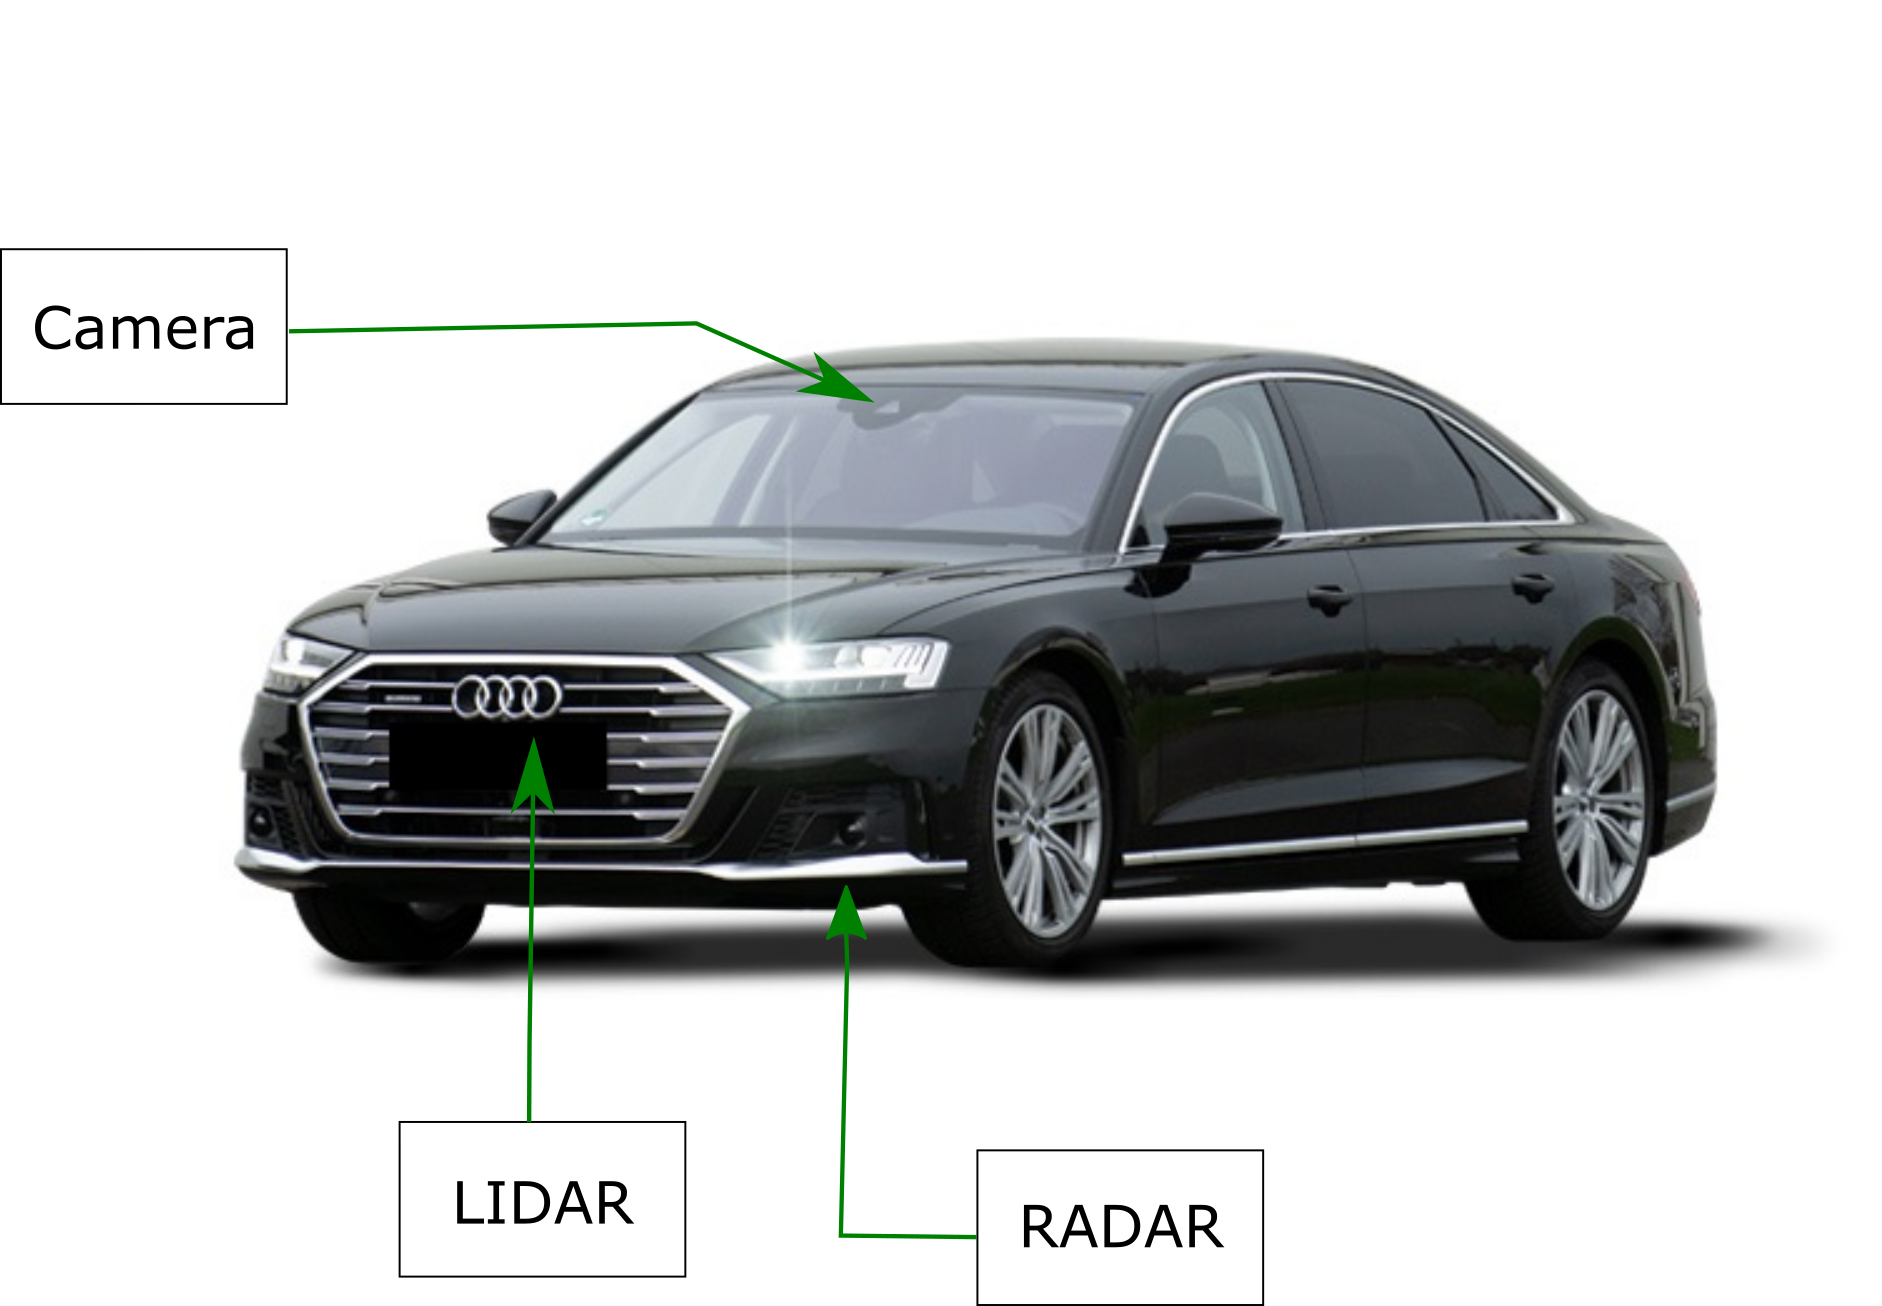
\includegraphics[scale=0.7]{imagens/image823.png}
\caption{Representation of an autonomous vehicle}
\label{fig:autonomous-vehicles}
\end{figure}


\subsection{Camera}
The camera is a type of sensor that allows the car to note the environment using the collected images. Figure \ref{fig:camera} shows the standard camera for autonomous vehicles.

It is an optical instrument for image or video capture in the same size. For example, there are some cameras where it is possible to set up the numbers of frames per second (FPS) and the image resolution. 

It is also essential to remember the importance of the camera's calibration; the Equations for this process were available in \cite{888718}. This step is necessary to acquire the objects' real size because it is sometimes required to compare these objects' dimensions. 

\begin{figure}[H]
\centering
\includegraphics[width=\columnwidth]{imagens/camera.png}
\caption{Representation of a camera of the autonomous vehicle}
\label{fig:camera}
\end{figure}

This sensor allows the car to detect many objects while it is possible to perform object recognition. It is necessary to freeze the difference between object detection and object recognition. There are different algorithms to perform these tasks. The proposed algorithm in Chapter \ref{capitulo4} shows both exposures combined with the estimation of the distance. 

\subsection{Radar}

The automotive radio detection and ranging (RADAR) sensors are responsible for performing object detection around the vehicle and avoiding potential collisions. Therefore, with this sensor, it is possible to warn the driver and combined with level 1 of automation, as shown in Figure \ref{fig:automation}, to intervene with the brake the car or use other controls to prevent an accident \cite{ariyur2006collision}.

\begin{figure}[H]
\centering
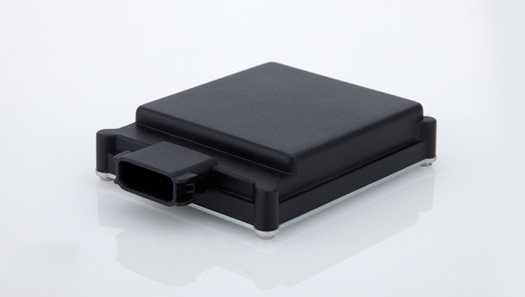
\includegraphics[width=\columnwidth]{imagens/radar.jpg}
\caption{A commercial radar model ARS430 CV from Continental}
\label{fig:camera}
\end{figure}

Another exciting application of the RADAR in the automotive scenario is measuring the relative speed to the vehicle and other objects. It is possible to estimate the distance correctly  \cite{stevenson2011long}.

It is possible to combine the camera and RADAR and get a new kind of sensor, as defined in \cite{kamerad}. With this approach, it is possible to reach 160 times faster than a human driver.

\subsection{Lidar}
In Figure \ref{fig:lidar} is shown a light detection and ranging (LIDAR). The main purpose of this laser is to detect and track any kind of objects. 
\begin{figure}[H]
\centering
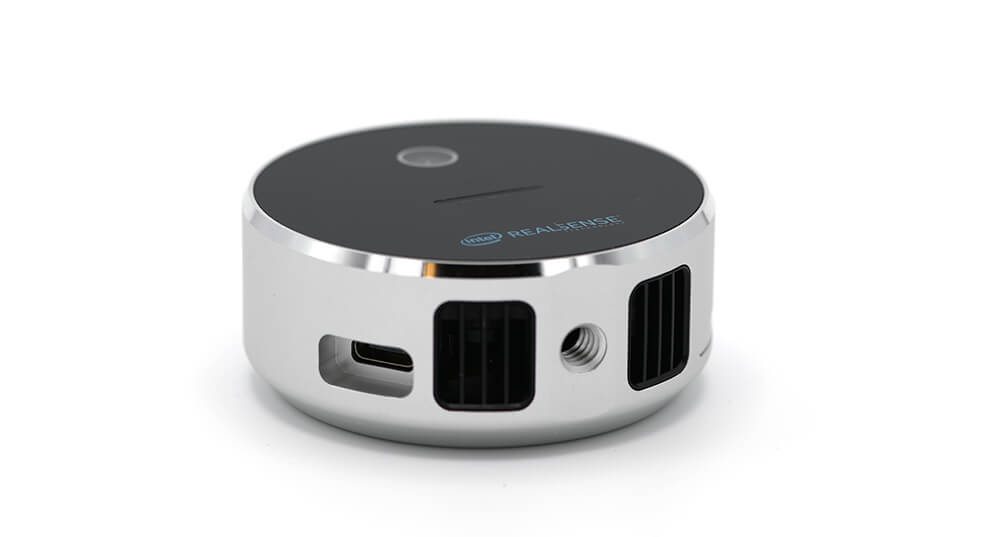
\includegraphics[width=\columnwidth]{imagens/lidar.jpg}
\caption{An exemple of a lidar of the autonomous vehicle}
\label{fig:lidar}
\end{figure}

This measurement is based on many times rotate this sensor in different directions, to scan the whole area of the autonomous vehicles is driving and collect some data for detecting the objects \cite{gao2018object}.

\section{Machine Learning}\label{ml-ai}
The machine learning is an approach based on algorithms to create some predictions. These techniques are based on mathematical and computer science. It is possible to apply this in several fields of science. 
\subsection{Artificial Neural Networks}

The human brain has inspired artificial neural networks (ANN) or perceptron. This approach is because of the capacity of the human mind to categorize new information. In Figure \ref{fig:ann} is shown an example of the structure of an ANN. There is an input array with the processed features for categorization. The next step of the processing is to define the weights for this analysis. The activation function is the central part of this process. In this step, the algorithm will transform the numbers collected by the previous actions and return only in twofold purpose, like $0$ and $1$ in the output layer \cite{goodfellow2016deep}.

\begin{figure}[H]
\centering
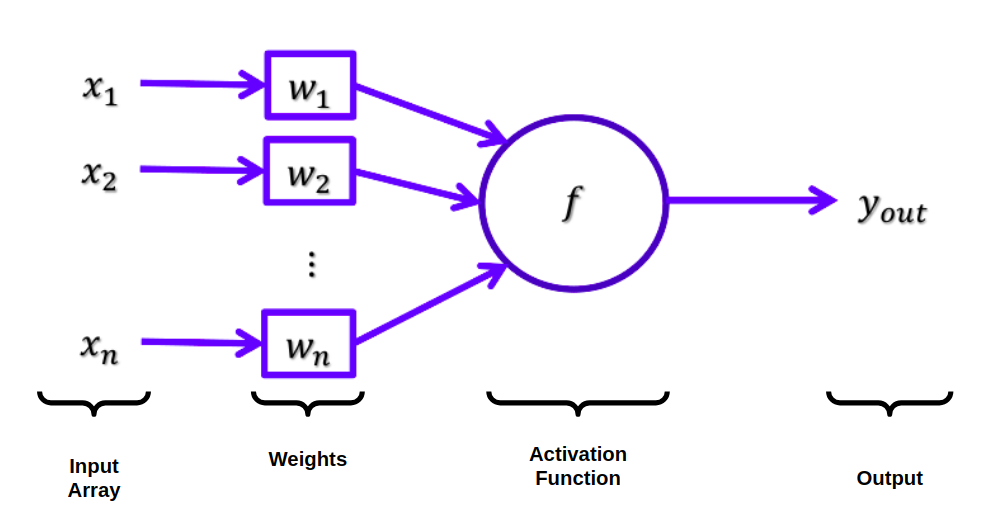
\includegraphics[width=\columnwidth]{imagens/ann.png}
\caption{The structure of an ANN \cite{lecture}}
\label{fig:ann}
\end{figure}

So, mathematically, the neuron output is a function of the weighted sum of its inputs. Figure \ref{fig:ann_weight} is shown the mathematical background. Where $f$ is activation function, $w_i$ are the weights, and $\beta$ is the constant input called bias.


\begin{figure}[H]
\centering
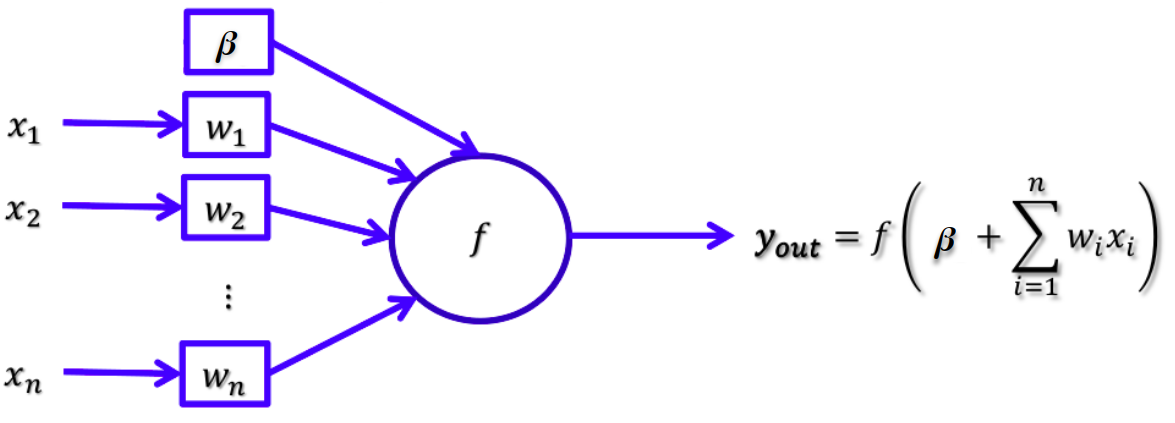
\includegraphics[width=\columnwidth]{imagens/math_ann_bias.png}
\caption{Mathematical representation of ANN with bias \cite{lecture}}
\label{fig:ann_weight}
\end{figure}


\subsubsection{Activation functions}
There are many different activation functions to use. These are crucial for ANN characteristics, such as learning ability and computational efforts in training and validation.

\begin{itemize}
    \item Unit step function
    \item Sign function
    \item Identity function
    \item Sigmoid function
    \item Hyperbolic tangent function
    \item Retified linear unit (Relu) 
\end{itemize}

\begin{table}[H]
\label{tab:tab1} 
\caption{Comparison Table for Activation Functions}
\centering
\resizebox{15.3cm}{!}{%
\begin{tabular}{|c|c|c|c|c|c|c|}
\hline
\textbf{\begin{tabular}[c]{@{}c@{}}Activation\\ Function\end{tabular}}  & \textbf{Linear}          & \textbf{Monotonic} & \textbf{Continuous}      & \textbf{\begin{tabular}[c]{@{}c@{}}Derivative \\ Monotonic\end{tabular}} & \textbf{\begin{tabular}[c]{@{}c@{}}Derivative\\ Continuous\end{tabular}} & \textbf{\begin{tabular}[c]{@{}c@{}}Simetric with \\ respect to \\ The Origin\end{tabular}} \\ \hline
{\color[HTML]{000000} Unit Step} & {\color[HTML]{FE0000} x} & {\color[HTML]{009901} \checkmark}& {\color[HTML]{FE0000} x} & {\color[HTML]{FE0000} x} & {\color[HTML]{FE0000} x} & {\color[HTML]{FE0000} x} \\ \hline
Sign & {\color[HTML]{FE0000} x} & {\color[HTML]{009901} \checkmark}& {\color[HTML]{FE0000} x} & {\color[HTML]{FE0000} x} & {\color[HTML]{FE0000} x} & {\color[HTML]{009901} \checkmark} \\ \hline
Identity & {\color[HTML]{009901} \checkmark}& {\color[HTML]{009901} \checkmark}& {\color[HTML]{009901} \checkmark}& {\color[HTML]{FE0000} x} & {\color[HTML]{009901} \checkmark}& {\color[HTML]{009901} \checkmark}\\ \hline
Sigmoid                                                                 & {\color[HTML]{FE0000} x} & {\color[HTML]{009901} \checkmark}             & {\color[HTML]{009901} \checkmark}                   & {\color[HTML]{FE0000} x}                                                 & {\color[HTML]{009901} \checkmark}                                                                   & {\color[HTML]{FE0000} x}                                                               \\ \hline
\begin{tabular}[c]{@{}c@{}}Hyperbolic\\ Tangent\end{tabular}            & {\color[HTML]{FE0000} x} & {\color[HTML]{009901} \checkmark}             & {\color[HTML]{009901} \checkmark}                   & {\color[HTML]{FE0000} x}                                                 & {\color[HTML]{009901} \checkmark}                                                                   & {\color[HTML]{009901} \checkmark}                                                                                 \\ \hline
\begin{tabular}[c]{@{}c@{}}Rectified \\ Linear Unit \\ (ReLU)\end{tabular} & {\color[HTML]{FE0000} x} & {\color[HTML]{009901} \checkmark}              & {\color[HTML]{009901} \checkmark}                   & {\color[HTML]{009901} \checkmark}                                                                   & \begin{tabular}[c]{@{}c@{}}{\color[HTML]{FE0000} x}\\ (at 0)\end{tabular}                       & {\color[HTML]{FE0000} x}                                                               \\ \hline
\end{tabular}}
\end{table}

In this work, Relu is the activation function chosen activation. Its mathematical definition is show in (\ref{eq:relu}). 


\begin{equation}
\label{eq:relu}
    f(x) = \mathrm{R}(x) = \mathrm{max}(0,x)
\end{equation}


The graphic visualization of the function Relu is shown in Figure \ref{fig:relu}, where this function returns $0$ if the number from the weighted sum is lower than $0$, or return $x$ if the previous value is over than $0$.


\begin{figure}[H]
\centering
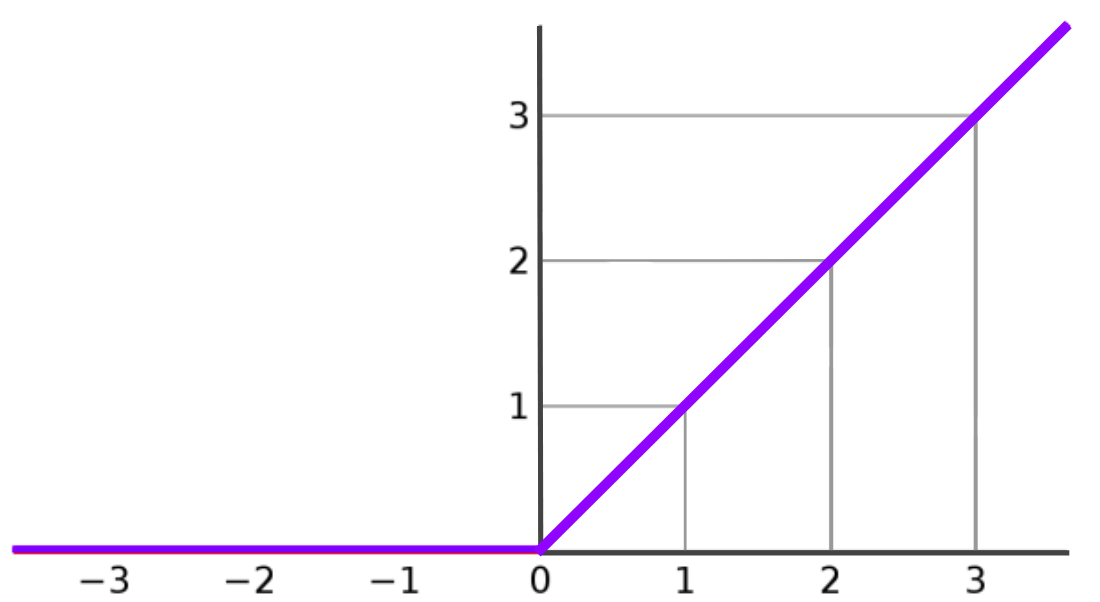
\includegraphics[scale=0.3]{imagens/relu_corrected.png}
\caption{The behavior of the Relu \cite{lecture}}
\label{fig:relu}
\end{figure} 

These are the essential characteristics of this activation function.

    \begin{itemize}
        \item Widely used in deep networks
        \item Pros: nonlinear, monotonic, derivative monotonic, and fast convergence
        \item Cons: not continuously differentiable at zero, i.e. issues with gradient descent around origin.
    \end{itemize}

\subsubsection{Layered Neural Networks}

The quintessential illustration of a deep learning model is the multilayer perceptron (MLP). An MLP is just a mathematical function mapping some set of input values to output values. The function
is formed by composing many more specific functions \cite{goodfellow2016deep}.


These are important deep learning models. The goal
of a feedforward network is to approximate some function $f*$. For example, for a classifier, $y = f*(x)$ maps an input x to a category y. A feedforward network
defines a mapping $y = f (x; \theta)$ and learns the value of the parameters $\theta$ that result in the best function approximation.

These models are called feedforward because information flows through the function being evaluated from $x$, through the intermediate computations used to define $f$, and finally to the output $y$. There are no feedback connections in which results of the model are fed back into itself.



\subsection{Convolutional Neural Networks}\label{sec:cnn}


The Convolutional Neural Networks (CNN) is a specialized kind of neural network for processing data known as in \cite{lecun1995convolutional}. For example, in the autonomous vehicle domain, this approach is several used for object detection and object identification. This name  indicates that the network employs a mathematical operation called
convolution. 

A CNN coarsely scans the image for features (in lower dimension space), pools possible patterns, then inspect those patterns in detail with its fully connected
subnetworks, generating their classifications. In Figure \ref{fig:cnn_car} is defined the full process of this neural network. Where there are three other importants is steps: Convolutional layer is defined in Subsection \ref{sub:conv}. The pooling layer is introduced in the Subsection \ref{sub:pooling}.
\begin{figure}[H]
\centering
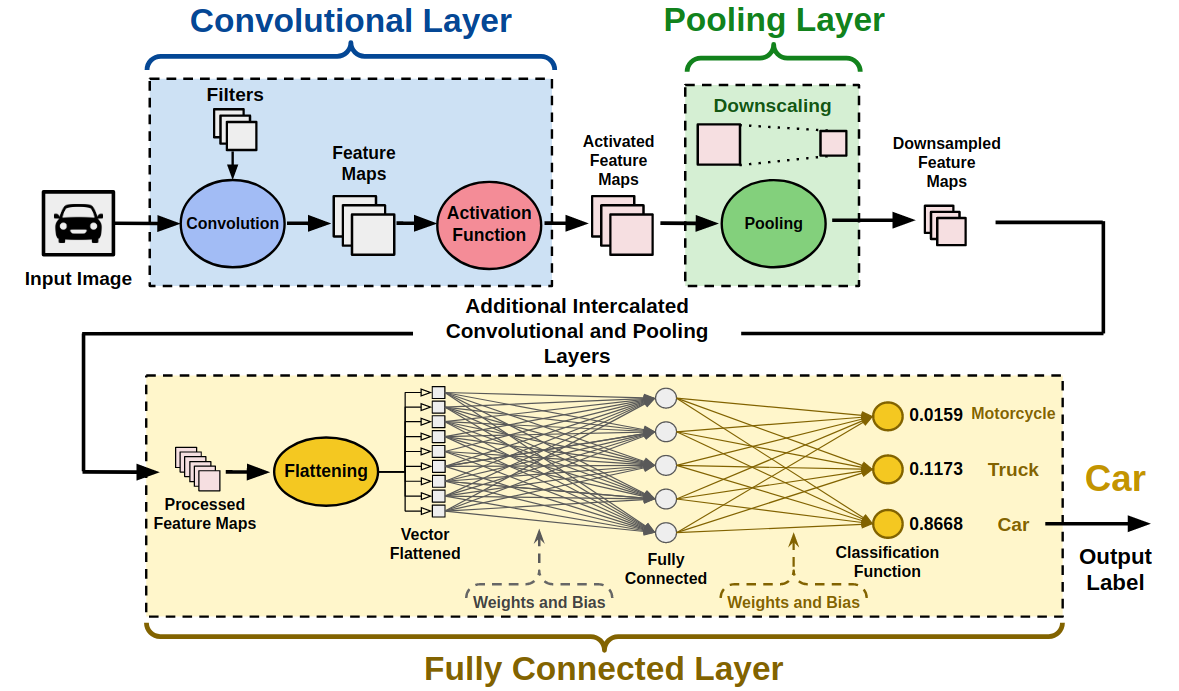
\includegraphics[width=\columnwidth]{imagens/Full_Process.png}
\caption{Full process of a convolutional neural network \cite{lecture}}
\label{fig:cnn_car}
\end{figure}


\subsubsection{Convolutional Layer}
\label{sub:conv}

The standard inputs are a tridimensional matrix with height and width defined accordingly with the image dimensions and determined by the number of colors. In general, the images use three color channels, Red-Green-Blue (RGB), as is shown in Figure \ref{fig:rgb}.

\begin{figure}[H]
\centering
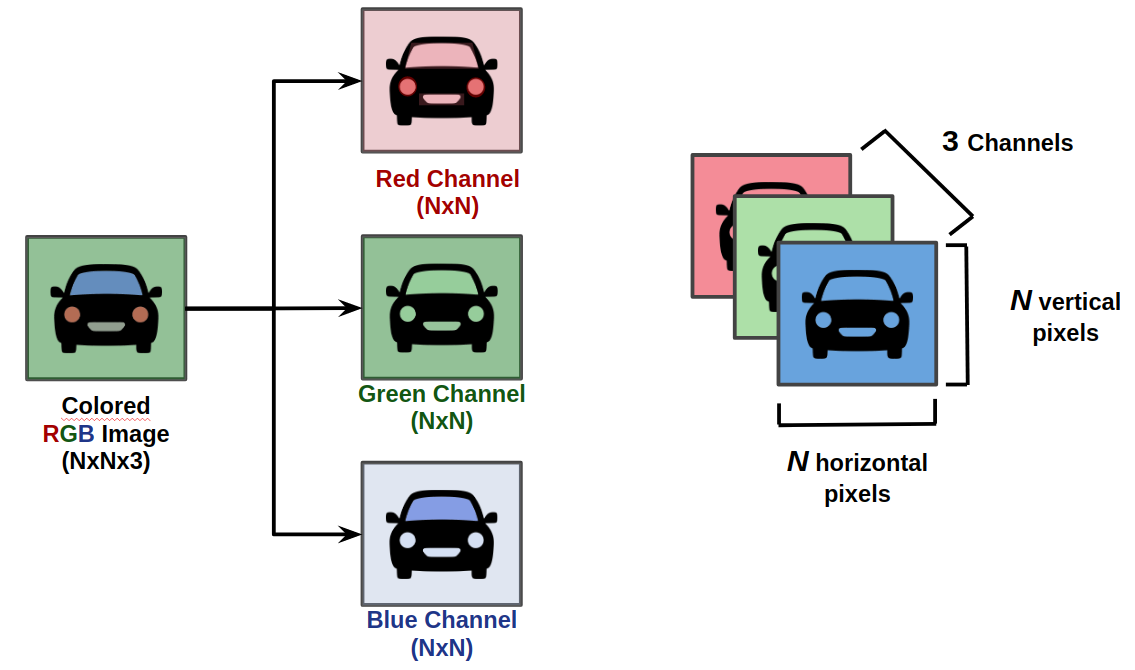
\includegraphics[scale=0.35]{imagens/rgb_representation.png}
\caption{Representation of the colors of the input image \cite{lecture}}
\label{fig:rgb}
\end{figure}


The convolutions work as filters that seem little squares, and they are slipping through the whole image and capturing essential parts.  Figure \ref{fig:bias} shows an image by dimensions of $NxNX3$, filter among the $MxMX3$, wherever individual main difference per result is then summed, on bias ($\beta$) value, then passed through an activation function. Furthermore, the end of the process generates a new matrix called a feature map or activation map.


\begin{figure}[H]
\centering
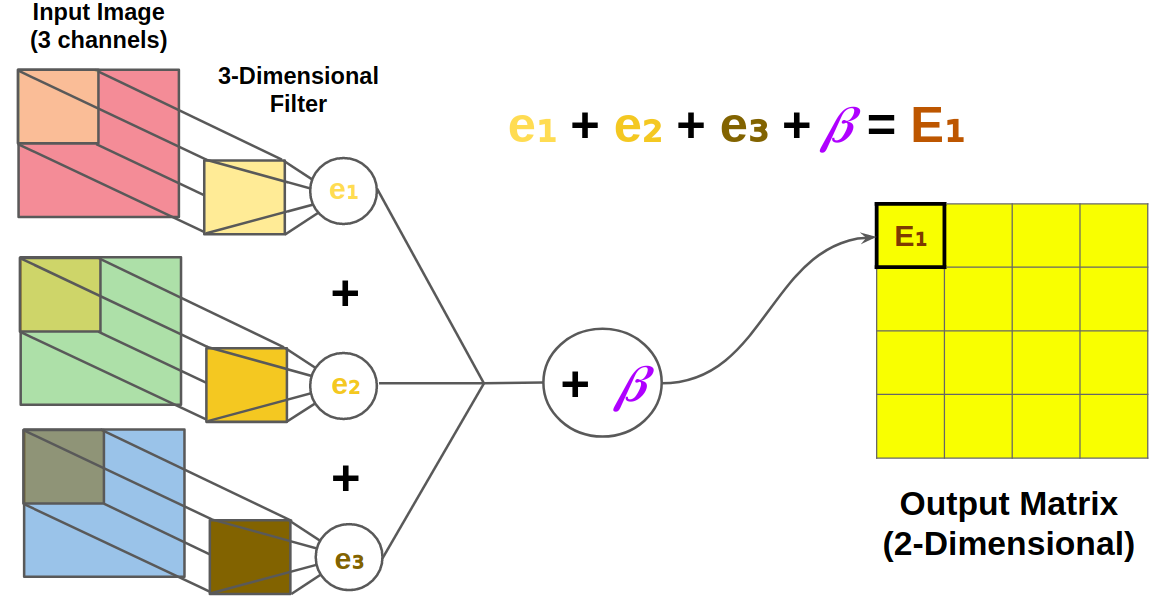
\includegraphics[scale=0.35]{imagens/three_dim_conv_2.png}
\caption{Representation of the convolution process \cite{lecture}}
\label{fig:bias}
\end{figure}




\subsubsection{Pooling and Upsampling}\label{sub:pooling}

A pooling layer is necessary to simplify the information from the previous layer. As happens with the convolution layer, it is choosing a unit area, for example, $2x2$ to slicing for the whole output information from the previous step. To brief, if the information from the previous layer was $4x4$, the output from the process of pooling will be $2x2$. Nevertheless, the most used method is max-pooling, where the biggest number in the matrix is passed to the next step. This data summarization is used to reduce the number of weights and avoid overfitting. In Figure \ref{fig:pooling} is shown the max-pooling process.

\begin{figure}[H]
\centering
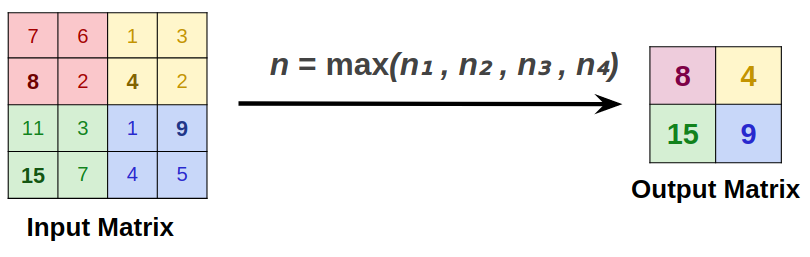
\includegraphics[scale=0.35]{imagens/max_pooling.png}
\caption{Representation of the maxpooling process \cite{lecture}}
\label{fig:pooling}
\end{figure}




\subsubsection{Auto-encoders}\label{auto-encoder}

It is a special type of neural network that is used to copy its inputs to its output. The intern structure is defined in Figure \ref{fig:autoencoder}. 

\begin{figure}[H]
\centering
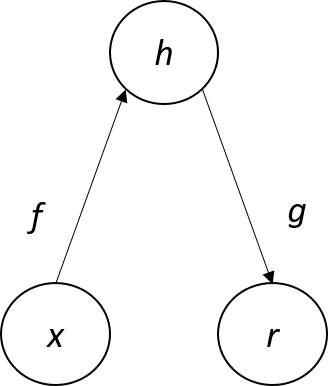
\includegraphics[scale=0.7]{imagens/autoencoder.png}
\caption{The structure of a standard autoenconder, where the variable $x$ means input and $r$ as an output through the internal representation in $h$. The encoder $f$ maps $x$ to $h$ and decoder $g$ maps $h$ to $r$}
\label{fig:autoencoder}
\end{figure}

As described in \cite{yang2020feedback}, this architecture has a hidden layer of $h$ that describes a code used to represent the input. The network may be viewed as consisting of two parts: an encoder function $h=f(x)$ and a decoder that produces a reconstruction $r=g(h)$.

\subsubsection{Training}

In the machine learning scenario, in special, the neural networks domain epoch can be defined as a single forward pass and backward pass of all the training examples. It feeds in all the neurons into the network at once. Instead, it chooses a batch of neurons and feeds them in. It performs stochastic gradient descent, and prevent the system from overfitting. There is a difference between individual training step time and total training time \cite{pascanu2013difficulty}. 


\section{Autonomous Vehicles} \label{autonomous-vehicles}

This section will be discussed the importance of the autonomous vehicles domain and its applicability to the society, and the problems occurred as well. 

\subsection{What are autonomous vehicles}
Modern vehicles now have Advanced Driver Assistance Systems (ADAS)
which work at several levels of autonomy, with these levels being
outlined by the National Highway Traffic Safety Administration
(NHTSA). The levels range from 0, no-automation, to 5, full self-driving automation \cite{national2013preliminary}. An example of an ADAS is a parking system, proposed by \cite{krasner2016automatic}, that uses sensors to find the best way to maneuver a car into a parking space without driver input. Systems such as these are being used in modern semi-autonomous
vehicles as driver aids to hand over work from the driver to the
car’s systems \cite{schoning2006parklenkassistent}. As technology progresses, there will be a more
and more handover of control from the driver to the vehicle, level
Four of automation being the fully-autonomous state that is a main talking point in the automotive industry. The level 5 AV will
be able to self-drive anywhere ("full automation"), i.e., no cockpits,
drivers are not required to be fit to drive, and even they do not require a driving license (every person in a vehicle is a passenger).

There are many open datasets to allow new people to work with autonomous vehicles and hackathons as well. In the special the KITTI Dataset \cite{geiger2013vision} and NuScenes in \cite{caesar2020nuscenes}. These datasets provided data using GPS, Camera, RADAR, and LIDAR. 

\subsection{Challenges}

The cities are not preparing for autonomous vehicles at the same velocity as the industry. Based on the data provided by \cite{cutler2015many}, only 6\% of the biggest cities in the United States are considering creating the necessary infrastructure to work with this new reality.

The process of putting autonomous vehicles on the street is prolonged due to other problems taking care of the network issues, even 3G, 4G, or 5G, the conservation of the roads, and the most critical aspect regarding the legislation. 

The study and development of these applications will change many things in society even in the process sector until companies that work with delivery. Nevertheless, it is indispensable to control the traffic and reduce the accidents, It follows the World Health Organization (WHO) every year over 1 million people lose their lives in car accidents, and only in Brazil is over 47,000 deaths \cite{world2004world}. 
